%\documentclass[a4paper,doc]{apa6}
\documentclass[a4paper]{article}
% \graphicspath{{/figures/}{./../figures/}}

\usepackage[english]{babel}
\usepackage[utf8x]{inputenc}
\usepackage{apacite}
\usepackage{authblk}  % for authors
\usepackage{xcolor}
\definecolor{mypink}{RGB}{255, 230, 255}

\usepackage{amsmath}
\usepackage{graphicx}
\usepackage[colorinlistoftodos,prependcaption]{todonotes}
\usepackage{pgfplotstable}
\pgfplotstableset{
	fixed zerofill,
	precision=3,
	col sep = comma,
	search path={../tables/}
}
\pgfkeys{/pgf/number format/precision=2, /pgf/number format/fixed}%

\newcommand{\getValue}[3]{%
	\pgfplotstablegetelem{#1}{#2}\of{#3}%
	\pgfmathprintnumber{\pgfplotsretval}%
}
\newcommand{\getCI}[2]{[\getValue{#1}{Lower}{#2}, \getValue{#1}{Upper}{#2}]}

\newcommand{\EJ}[1]{\todo[inline, color=green]{  #1 }}
\newcommand{\Q}[1]{\todo[inline, color=yellow]{  #1 }}
\newcommand{\jv}[2]{{\color{red}\st{#1}}{\color{blue}\bf{#2}}}
\newcommand{\DON}[1]{\todo[inline, color=orange]{#1}}
\newcommand{\DONside}[1]{\todo[color=orange]{#1}}
\newcommand{\J}[1]{\todo[inline, color=mypink]{#1}}

\graphicspath{{../figures/}}
\newcommand{\hypo}{\mathcal{H}}
\newcommand{\model}{\mathcal{M}}
\newcommand{\data}{\mathcal{D}}


\newcommand{\osflink}{\url{https://osf.io/uq8st/}}

\newcommand{\CamererReplication}{\url{https://mfr.osf.io/render?url=https://osf.io/fg4d3/?action=download\%26mode=render}}
\newcommand{\manyLabsLink}{\url{https://mfr.osf.io/render?url=https://osf.io/xufw4/?action=download\%26mode=render}}

\title{A Cautionary Note on Estimating Effect Sizes with Confidence Intervals}
%\shorttitle{Estimating Effect Size} 
\renewcommand{\thefootnote}{\fnsymbol{footnote}}
\author[1]{Don van den Bergh%
	\thanks{Correspondence concerning this article should be addressed to: Don van den Bergh, University of Amsterdam, Department of Psychological Methods, Nieuwe Achtergracht 129B, 1018VZ Amsterdam, The Netherlands. E-Mail should be sent to: donvdbergh@hotmail.com.
}}
\author[1]{Julia M. Haaf}
\author[1,2]{Alexander Ly}
\author[3]{\authorcr Jeffrey N. Rouder} % putt Jeff on a newline to avoid a newline after his first name
\author[1]{Eric-Jan Wagenmakers}
\affil[1]{University of Amsterdam}
\affil[2]{Centrum Wiskunde \& Informatica}
\affil[3]{University of California Irvine}
\date{}
%\affiliation{~}
\renewcommand*{\thefootnote}{\arabic{footnote}}
%
%\threeauthors{Don van den Bergh and Julia M. Haaf and Alexander Ly and Eric-Jan Wagenmakers}{Alexander Ly}{Jeffrey N. Rouder}
%\threeaffiliations{University of Amsterdam}{Centrum Wiskunde \& Informatica}{University of California Irvine}
%\authornote{Correspondence concerning this article should be addressed to: Don van den Bergh, University of Amsterdam, Department of Psychological Methods, Nieuwe Achtergracht 129B, 1018VZ Amsterdam, The Netherlands. E-Mail should be sent to: donvdbergh@hotmail.com.}


%TODO:
%
% - Idee Jeff: Figure 95% posterior predictive for a single point model averaged?
% - data from https://osf.io/pfdyw/  ?

\begin{document}
\pgfplotstableread{effectSizeExample.csv}\tbEffectSizeExample
	\section*{Outline}

\paragraph{Introduction}
\begin{itemize}
	\item Introduce an example about reporting effect size + confidence interval (with data, preferably a t-test). 
	\item Reference some editorials + papers on the topic.
	\item Pop the question: Given the data, what is the best estimate of effect size?
\end{itemize}
\paragraph{Ignoring Model Uncertainty Leads to Overestimating Effect Size}
\begin{itemize}
	\item There are many reasons why effect size is overestimated. Mention some reasons that will not be discussed (e.g., publication bias) and some that will be discussed (ignoring model uncertainty).
	\item Make the argument that since model uncertainty is considered initially, this uncertainty should propagate to parameter estimates.
	\item Relate this argument to model averaging and its successes.
	\item Reanalyze the data example from the introduction but model average over H0 and H1.
\end{itemize}
\paragraph{Discussion}
\begin{itemize}
	\item When not to model average:
	\begin{enumerate}
		\item when models are theoretical opposites.
		\item statistically different (e.g., uninterpretable)
		\item don't have to model average but instead use spike and slab model
	\end{enumerate}
	\item say you can only report one number? Then we recommend the model averaged estimate + Bayes factor
\end{itemize}

\newpage
\listoftodos

\newpage
\maketitle

\begin{abstract}
	content...
\end{abstract}

\newpage
Your colleague has just conducted an experiment for a registered report. The analysis yields $p<0.05$ and your colleague believes that the null hypothesis can be rejected. In line with recommendations both old \cite<e.g., >{Grant1962, Loftus1996} and new \cite<e.g., >[NEJM editorial!]{Cumming2014} you convince your colleague that it is better to replace the $p$-value with an estimate of effect size and a 95\% confidence interval \cite<but see>{MoreyEtAl2016CI}. You also manage to convince your colleague to plot the data. Instead of simply reporting $p<.05$, the statistical analysis in the report is now more informative. The result is shown in Figure~\ref{fig:descriptivesPlot}. In the text of the paper, the result is summarized as Cohen's $d = \getValue{0}{Estimate}{\tbEffectSizeExample}$, CI $= \getCI{0}{\tbEffectSizeExample}$.

\begin{figure}[!ht]
	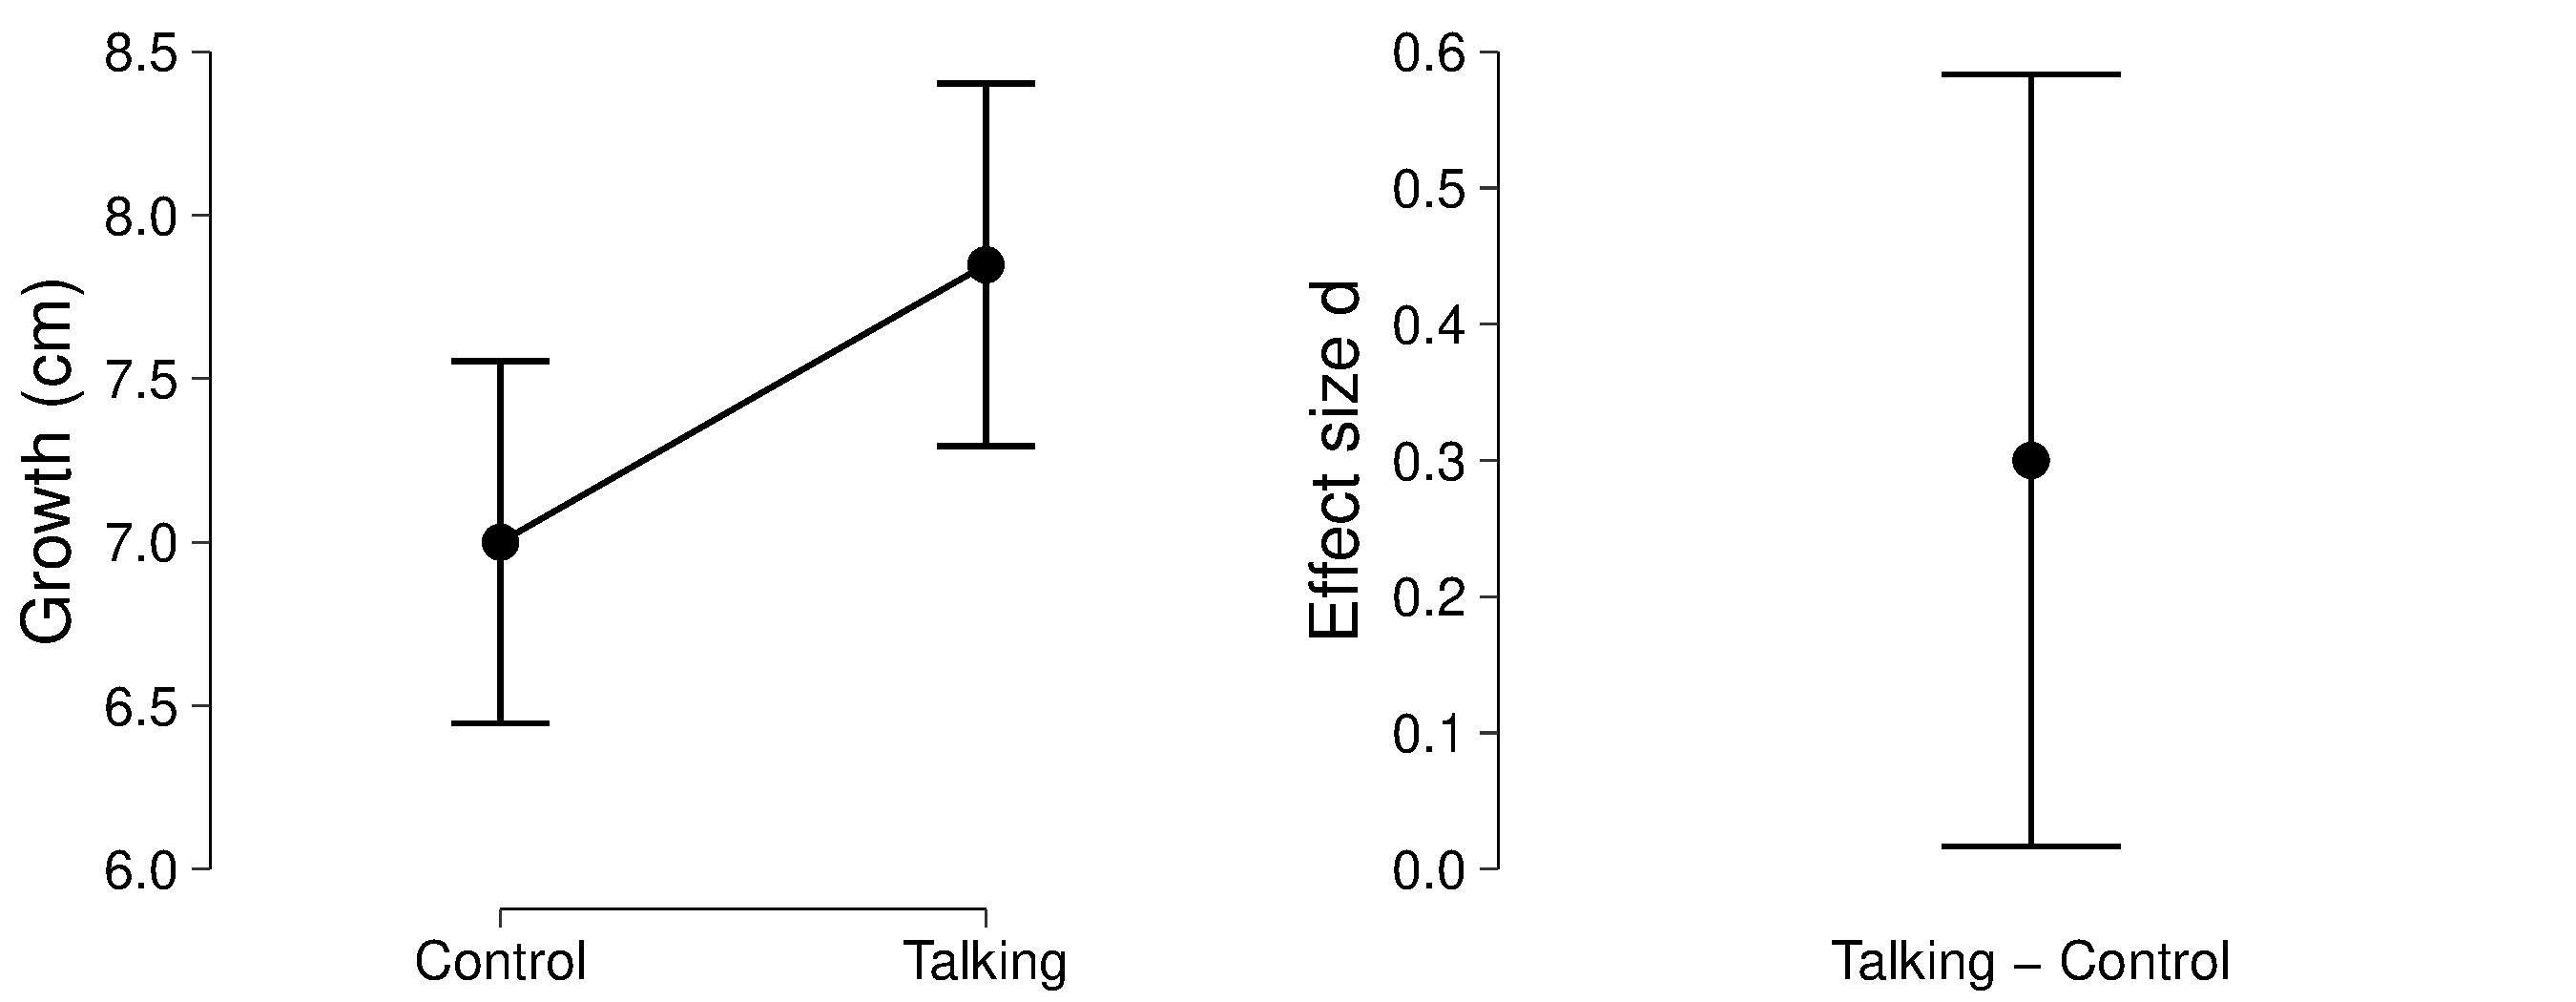
\includegraphics[width=\textwidth]{descriptivesPlot.pdf}
	\caption{The left panel shows a box plot with the observations as gray dots. The right panel shows an estimate of the effect size, Cohen's d, and a 95\% confidence interval. The data were simulated.}
	\label{fig:descriptivesPlot}
\end{figure}

Given the results shown in Figure~\ref{fig:descriptivesPlot}, what is the best point estimate of effect size? An obvious answer is ``\getValue{0}{Estimate}{\tbEffectSizeExample}''; since the confidence interval does not contain 0, the sample effect size seems to be a reasonable choice. However, your colleague now tells you about the nature of the experiment: plants grow faster when you talk to them. Suddenly, an effect size of ``0'' also appears plausible.\footnote{Unless you pray out loud, with consumption, and the plant is near.}

Although some may argue that all null hypothesis are false \cite[?]{Cohen1994}, several large-scale replications studies have demonstrated that an effect size of zero is reasonable \cite<e.g., see the meta analyses conducted by>{KleinEtAl2018ML2, CamererEtAl2018, NosekLakens2014}.

\section*{When Effect Sizes are Overestimated}

Given a limited sample size, a point estimate of effect size and a confidence interval tend to overestimate the true effect size. To illustrate, we reanalyze the simulated data from Figure~\ref{fig:descriptivesPlot}. There are two hypotheses considered: The null hypothesis which states that the two groups have the same population mean and the alternative hypothesis that states the two groups differ in their population mean. For simplicity, we test these hypothesis using a two-sample t-test. Traditionally, one decides upon a single model using some form of significance testing. Assuming the the alternative model comes out victorious, it is then used to obtain estimates of effect size and predictions for future observations. However, it has been shown repeatedly that model averaging provides the best predictive performance (\citeNP[pp. 640-641]{ZellnerVandaele1975}, as described in \citeNP[p. 600-601]{ZellnerSiow1980}; \citeNP[p. 57]{Haldane1932}, \citeNP{IversonEtAl2010}, \citeNP{RouderEtAl2018PBR}), and conceptually similar ideas date back much further (\citeNP[p. 387]{WrinchJeffreys1921}, \citeNP{Jevons18741913}). Accordingly, an estimate of the model averaged effect size can be obtained by averaging the effect size of the null model and that of the alternative model by the posterior probabilities of both models. This yields $p(\delta\mid\data) = 0 pr(\model_0\mid\data) + p(\delta\mid\data,\model_1)pr(\model_1\mid\data)$.\DONside{Let d be the effect size of the model averaged posterior predictive distribution. Consider the limit of d as the number of posterior predictive observations goes to infinity. Do we retrieve the model averaged posterior effect size? Intuitively yes, which could be a nice argument that the model averaged effect size can definitely be interpreted for this model.} Figure~\ref{fig:modelAveragedPosterior} shows both the model averaged posterior of effect size and the posterior effect size under $\model_1$.

%With sparse data, the prior distribution shrink the estimate towards its mean, in this case 0.\DON{I know the prior shrinks estimates towards 0, but this has little to do with the true effect size. Rather, it's a reason why Bayesian estimators (of effect size) are be biased and tend to underestimate the true value.}
% In addition, since the null hypothesis is considered a-priori plausible, its predictions should be considered also. It has been shown repeatedly that model averaging provides the best predictive performance (\citeNP[pp. 640-641]{ZellnerVandaele1975}, as described in \citeNP[p. 600-601]{ZellnerSiow1980}; \citeNP[p. 57]{Haldane1932}, \citeNP{IversonEtAl2010}, \citeNP{RouderEtAl2018PBR}), and conceptually similar ideas date back much further (\citeNP[p. 387]{WrinchJeffreys1921}, \citeNP{Jevons18741913}). Thus, to obtain the best predictions one should model average over the null and alternative hypothesis. The impact of the null will shrink the estimate of effect size towards 0.
% 
% \J{We should probably first introduce the two relevant models here, and the idea that an unconstrained model is used for estimation. Maybe even say something like noone would use the null model to generate effect size estimates, why would we use the unconstrained?}


\begin{figure}[!ht]
	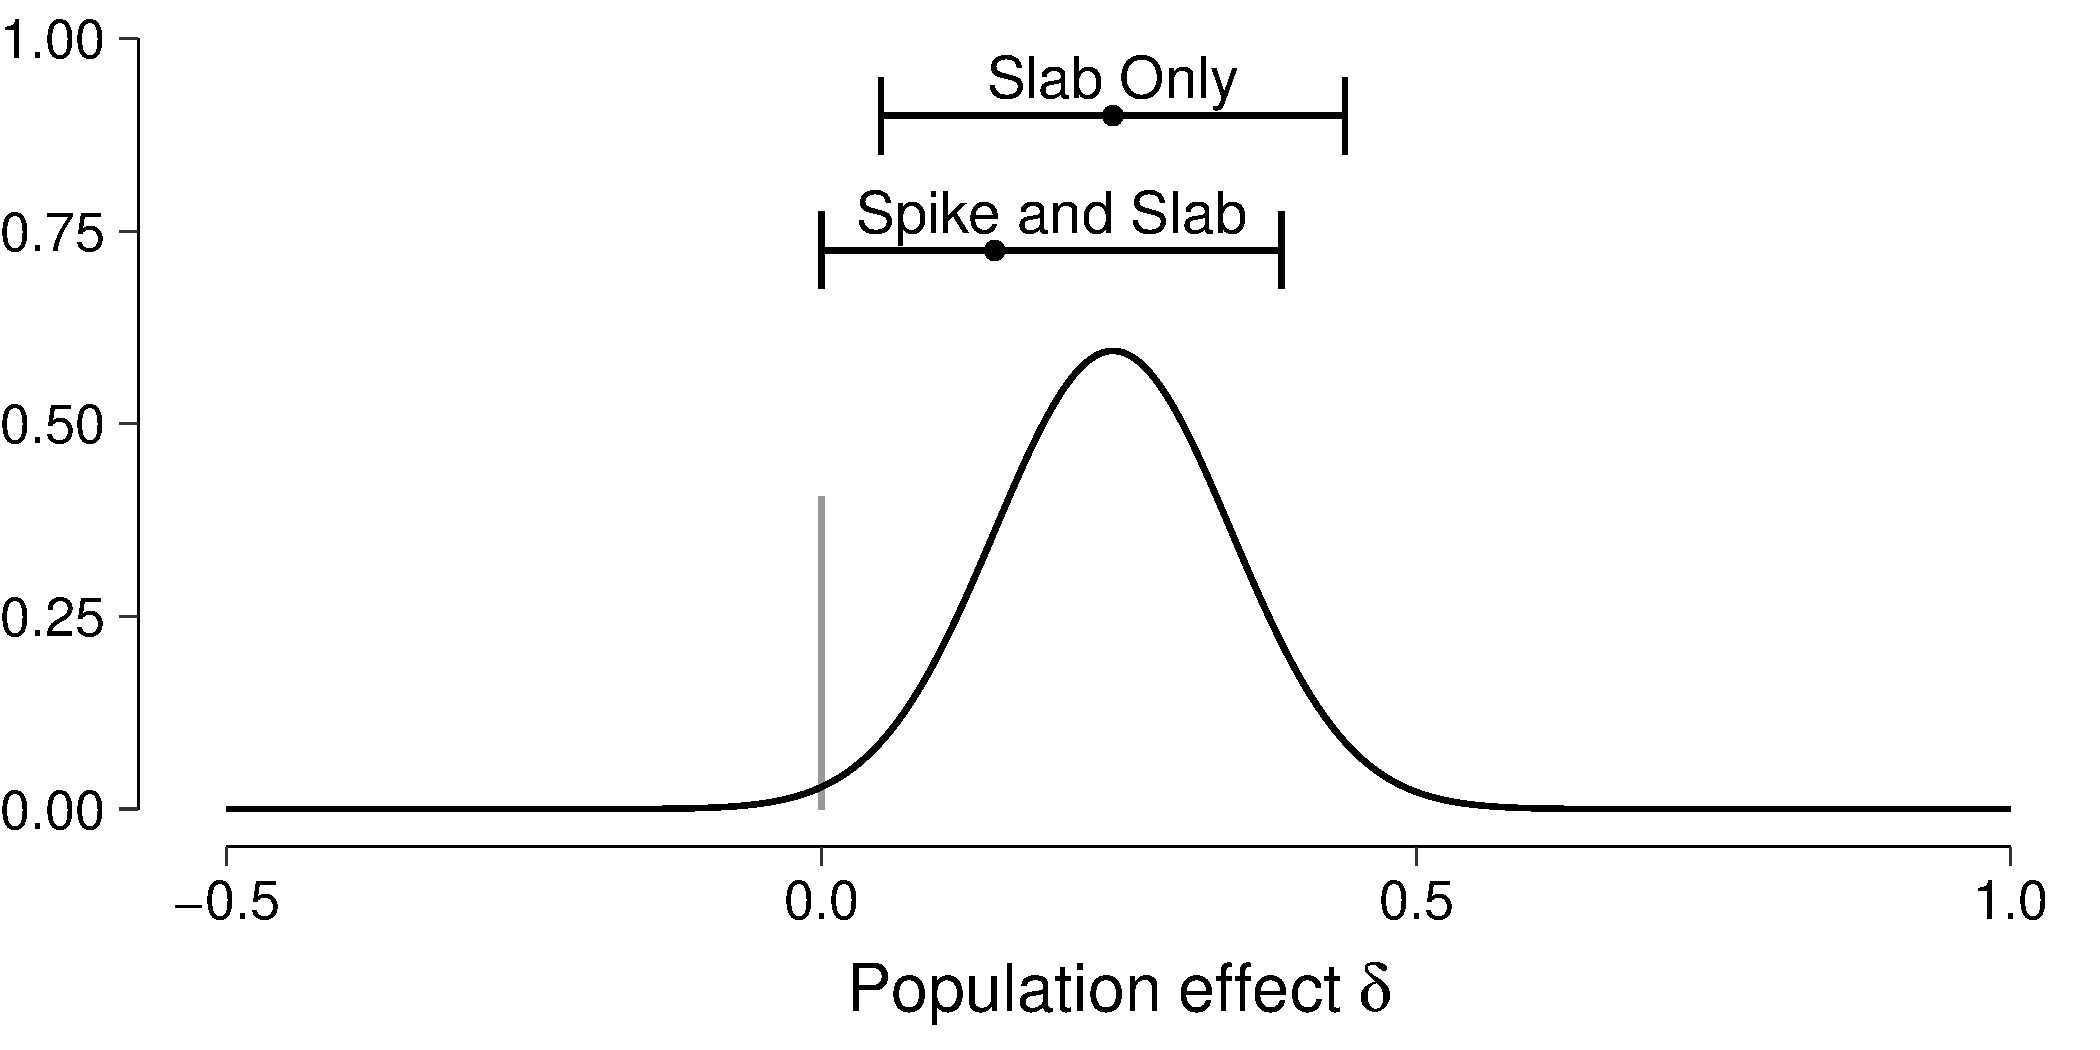
\includegraphics[width=\textwidth]{spikeAndSlabPosteriorRescaledPosteriorMode.pdf}
	\caption{A visualization of model averaging. The black line represents the posterior of the effect size given the alternative model (i.e., the slab). This posterior distribution integrates to the posterior probability of the model given uniform prior model probabilties. The grey line represent the posterior probability of the null model (i.e., the spike). The yellow error bar shows a 95\% central credible interval if inference is only based on the posterior under the slab. The purple error bar shows a 95\% central credible interval if inference is based on the model averaged posterior distribution. %Although there is substantial uncertainty about the models ($p(\model_0\mid X) = p(\model_1\mid X) = 0.5$), an estimate based on only the posterior distribution of the alternative model may be overconfident and positively biased.
	\DON{Do we want a plot of the prior as well? That would be a bit close to Johnny's figure though.}}
	\label{fig:modelAveragedPosterior}
\end{figure}
The posterior density of effect size under null model is a spike and usually represented with a Dirac delta function. 
The model averaged posterior are shrunken more towards 0 than the pos


\begin{figure}[!ht]
	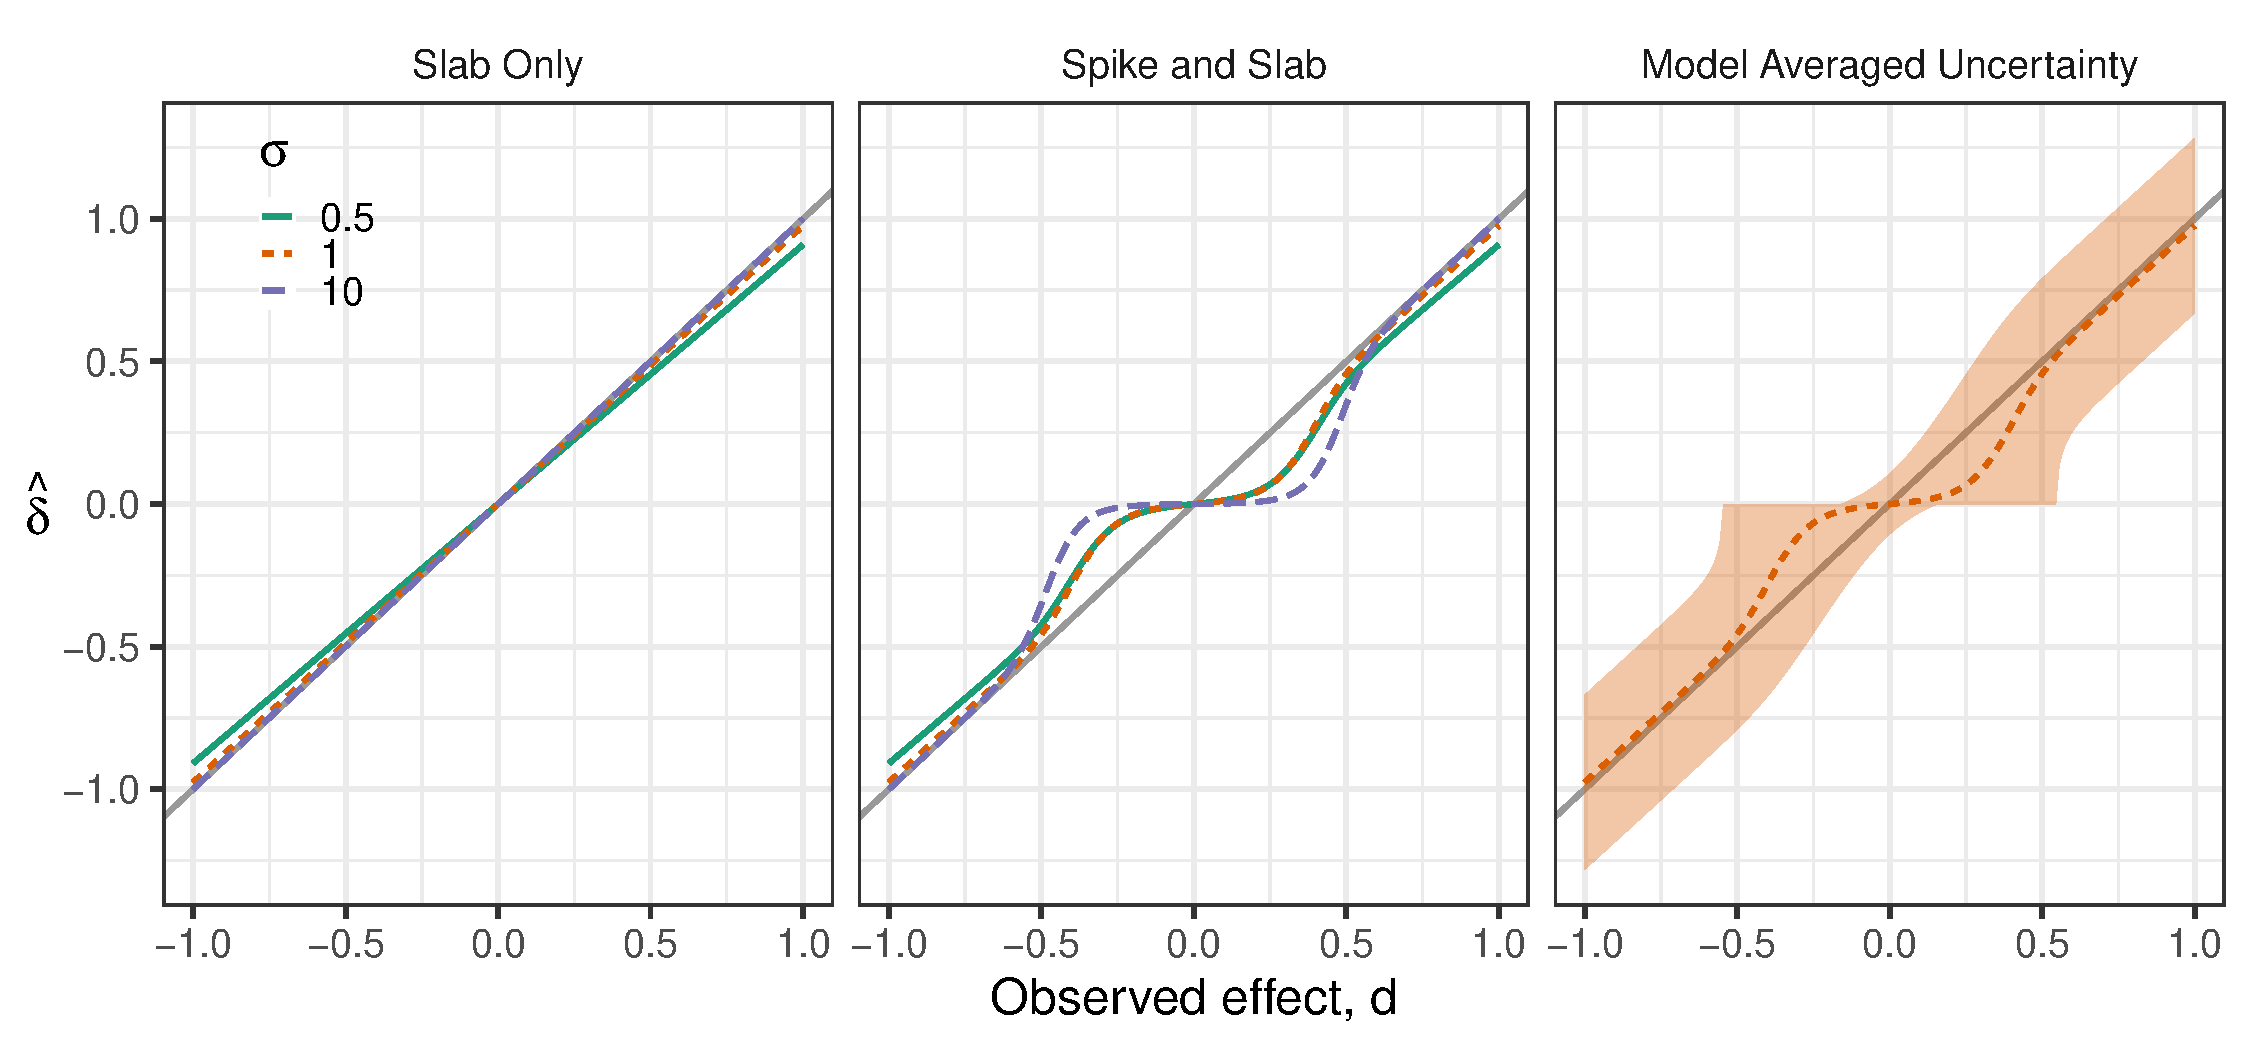
\includegraphics[width=\textwidth]{posteriorMeanVsSampleDelta3panel.pdf}
	\caption{Posterior mean for effect size (y-axis) as a function of the observed effect size (x-axis). The left panel shows inference conditional on the alternative model (i.e., the slab). The middle panel shows the model averaged posterior mean, which shrinks towards 0 as the sample effect size approaches 0 and the null model becomes more plausible. The right panel shows the a 95\% credible interval for the model averaged posterior. The colors and line types represent different variances of the prior distribution.}
	\label{fig:posteriorMeanVsSampleDelta}
\end{figure}


Show prior-posterior plot from JASP:
With sparse data, the prior distribution on effect size will shrink the estimate towards 0. Happens with the default settings, but even more when the width is smaller.

Also, show spike at zero (maybe we need better JASP plot, will ask Don to create it):

The impact of H0 will shrink the estimate toward 0. This is most clear when H0 is a priori very likely (''plants do not grow faster when you pray for them'') or when the sample effect is very close to zero, so that it becomes clear that H0 might provide a more reasonable explanation.

Mention earlier literature:
Model averaging effect size:
\cite[pp. 640-641]{ZellnerVandaele1975}, as described in \cite[p. 600-601]{ZellnerSiow1980}; also \cite[p. 57]{Haldane1932}, \cite{IversonEtAl2010}

Early ideas that are conceptually similar can be found in \cite[p. 387]{WrinchJeffreys1921} (show BMA between $\mathcal{H}_1$ and $\mathcal{H}_0$ -- but for prediction, not estimating effect size!; see also \cite{Jevons18741913}).

See also \cite{RouderEtAl2018PBR}:

Key is Figure 5. The spike-and-slab model shows shrinkage towards zero for small observed effect sizes because the spike has increased influence.

``There are alternative interpretations that we find somewhat cumbersome. One is that the spike-and-slab can be viewed not as a model but as a model-averaging device. Here, the goal is not so much to define categories of effect and no-effect, but to average across both of them, and this averaging results in regularization. If one uses this interpretation, the prior odds settings are important as they influence the posterior weight given to each model component in the averaging. Another alternative interpretation comes from Kruschke and Liddell (Kruschke, 2011; Kruschke \& Liddell, 2017; this issue). Here, the spike and slab are seen as separate components in a hierarchical model. Accordingly, a focus on Bayes factors denotes a focus on the choice between components; a focus on posterior estimation entails parameter estimation after choosing the slab. We find this view difficult inasmuch as there is no a priori reason to choose the slab to focus on estimation. If one admits the possibility of the spike, then assuredly it should affect posterior estimation as well.''

\section*{Discussion}

Bayesian estimators more likely to underestimate the effect size, as prior mean is typically centered around the null which pulls the posterior mean towards 0.

\subsubsection*{When not to model average}
\J{Which models to average? When to average? Also consider alternatively one model that has all relevant components for estimation instead of separate models.}

\newpage
\clearpage
\bibliographystyle{apacite}
\bibliography{referenties, referenties.bib}
%\clearpage

%\appendix
%\section{Bla}

\end{document}